%Grundlagen.tex

\section{Grundlagen}
\label{sec:Grundglagen}
\subsection{Ladung}
\label{sec:Ladung}

\begin{tabular}{l l}
	\begin{minipage}[l]{5cm}
		\[
			Q=I \cdot t
		\]	
		\[
			[Q]=C=As
		\]
	\end{minipage}
	&
	\begin{minipage}[l]{5cm}
		$Q$: Ladung \\
		$I$: Stromstärke \\
		$t$: Zeit
	\end{minipage}
\end{tabular}

\subsection{Stromdichte}
\label{sec:Stromdichte}

\begin{tabular}{l l}
	\begin{minipage}[l]{5cm}
		\[
			J=\frac{I}{A}
		\]
		\[
			[J] = \frac{A}{m^2}
		\]
	\end{minipage}
	&
	\begin{minipage}[l]{5cm}
		$J$: Stromdichte \\
		$I$: Stromstärke \\
		$A$: Leiterquerschnitt
	\end{minipage}
\end{tabular}	


\subsection{Strömungsgeschwindigkeit der Elektronen}
\label{sec:StrömungsgeschwindigkeitDerElektronen}

\begin{tabular}{l l}
		\begin{minipage}[l]{5cm}
		\[
		v=\frac{I}{e\cdot n\cdot A}
		\]
		\[
		[v]=\frac{m}{s}
		\]
		\end{minipage}
	&
	
	\begin{minipage}[l]{5cm}
		$v$: Stömungsgeschwindigkeit \\ 
		$I$: Stromstärke \\
		$e$: Elementarladung \\
		$n$: Elektronendichte \\
		$A$: Leiterquerschnitt
	\end{minipage}
\end{tabular}

\subsection{Spannung}
\label{sec:Spannung}
\begin{tabular}{l l}
	\begin{minipage}[l]{5cm}
		\[
		U=\frac{W}{Q}
		\]
		\[
		[U]=V=\frac{Nm}{As}=\frac{kg\,m^2}{As^3}
		\]
	\end{minipage}
&
	\begin{minipage}[l]{5cm}
		$U$: Spannung \\
		$W$: Energie /Arbeit \\
		$Q$: Ladung
	\end{minipage}
\end{tabular}

\subsection{Das ohmsche Gesetz (Widerstand)}
\label{sec:DasOhmscheGesetzWiderstand}

\begin{tabular}{l l}
	\begin{minipage}[l]{5cm}
		\[
		R=\frac{U}{I}
		\]
		\[
		[R]=\frac{V}{A}=\Omega
		\]
		\[
		G=\frac{I}{U}=\frac{1}{R}
		\]
		\[
		[G]=\frac{A}{V}=\frac{1}{R}=S
		\]
	\end{minipage}
	&
	\begin{minipage}[l]{5cm}
		$R$: Widerstand \\
		$G$: Leitwert \\
		$U$: Spannung \\
		$I$: Stromstärke 
	\end{minipage}
\end{tabular}

\subsection{Spezifischer Widerstand}
\label{sec:SpezifischerWiderstand}

\begin{tabular}{l l}
	\begin{minipage}[l]{5cm}
		\[
		R=\frac{\rho\cdot l}{A} = \frac{l}{\kappa\cdot A}
		\]
		\[
		[\rho]=\frac{\Omega \, m^2}{m}=\Omega \, m
		\]
		\[
		[\kappa]=\frac{1}{\Omega \, m}=\frac{S}{m}
		\]
		\[
		\kappa=\frac{1}{\rho}
		\]
	\end{minipage}
	&
	\begin{minipage}[l]{6cm}
		$\rho$: spezifischer Widerstand \\
		$l$: Länge des Leiters \\
		$A$: Querschnittsfläche des Leiters \\
		$\kappa$: spezifische Leitfähigkeit
	\end{minipage}
\end{tabular}


\subsection{Temperaturabhänigkeit des Widerstandes}
\label{sec:TemperaturabhänigkeitDesWiderstandes}

\begin{tabular}{l l}
	\begin{minipage}[l]{5cm}
		\[
		R_2=R_1[1+\alpha_1(\vartheta_2-\vartheta_1)]
		\]
	\end{minipage}
	&
	\begin{minipage}[l]{5cm}
		$R_1$: Widerstand bei $\vartheta_1$ \\
		$R_2$: Widerstand bei $\vartheta_2$ \\
		$\vartheta_1$: Ausgangstemperatur \\
		$\vartheta_2$: Endtemperatur \\
		$\alpha_1$: Temperaturkoeffizient 
	\end{minipage}
\end{tabular}


\subsection{Leistung und Arbeit(Energie)}
\label{sec:ArbeitUndLeistung}
\begin{tabular}{l l}
	\begin{minipage}[l]{6cm}
		\[
		P=U\cdot I=\frac{U^2}{R}=I^2\cdot R
		\]
		\[
		[P]=W=VA=\frac{J}{s}=\frac{kg \, m^2}{s^3}
		\]
		\[
		W=E=P\cdot t
		\]
		\[
		[W]=[E]=J=Ws=\frac{kg \,m^2}{s^2}
		\]
	\end{minipage}
	&
	\begin{minipage}[l]{5cm}
		$P$: Leistung \\
		$W$: Arbeit\\
		$E$: Energie\\
		$U$: Spannung\\
		$I$: Stromstärke
	\end{minipage}
\end{tabular}


\subsection{Wirkungsgrad}
\label{sec:Wirkungsgrad}

\begin{tabular}{l l}
	\begin{minipage}[l]{5cm}
		\[
		\eta=\frac{P_{ab}}{P_{zu}}
		\]
	\end{minipage}
	&
	\begin{minipage}[l]{5cm}
		$\eta$: Wirkungsgrad
	\end{minipage}
\end{tabular}


\subsection{Pfeilsysteme}
\label{sec:Pfeilsysteme}

\subsection{Umwandlung von Quellen}
\label{sec:UmwandlungVonQuellen}


\begin{figure}[H]
	\centering
%		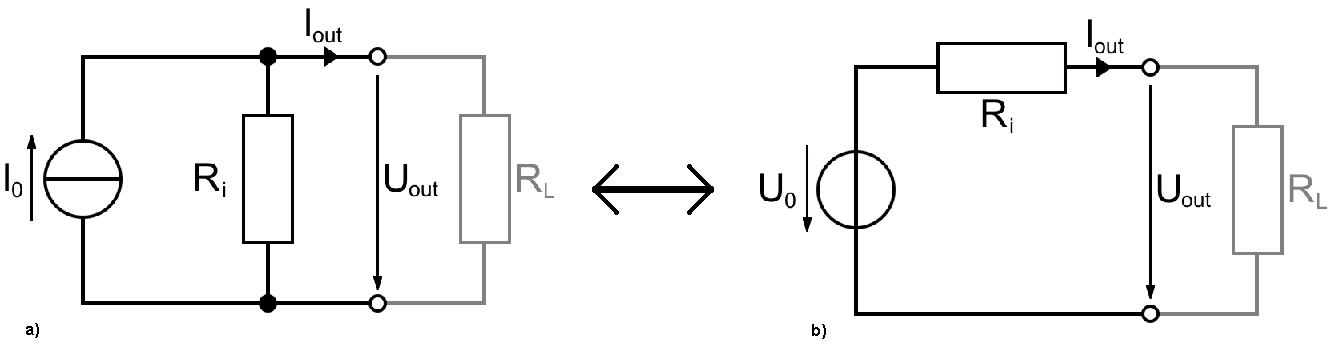
\includegraphics[width=8CM]{Grafiken/reale_Quellen.png}	
	\caption{reale Quellen mit Innenwiderstand}
	\label{fig:reale_Quellen}
\end{figure}


\begin{itemize}
	\item Bei der Umwandlung von Quellen zeigt der Pfeil der neuen Quelle entgegengesetzt der vorherigen Quelle. Siehe Abbildung \ref{fig:reale_Quellen} Seite 
\end{itemize}
\pageref{fig:reale_Quellen}

\paragraph{Stromquelle $\rightarrow$ Spannungsquelle}
\label{sec:StromquelleSpannungsquelle}
\[
U_q=I_q\cdot R_i
\]

\paragraph{Spannungsquelle $\rightarrow$ Stromquelle}
\label{sec:SpannungsquelleStromquelle}
\[
I_q=\frac{U_q}{R_i}
\]



\subsection{Die Kirchhoff'schen Gesetze}
\label{sec:DieKirchhoffSchenGesetze}

\subsubsection{Knotenregel}
\label{sec:Knotenregel (1. Kirchhoff'sches Gesetz}
Die Summe aller Ströme die in einen Knotenpunkt führen ist Null.
\[
\sum I_k = 0
\]

%(Bild)

\subsubsection{Maschenregel (2. Kirchhoff'sches Gesetz)}
\label{sec:Maschenregel}
Die Summe aller Spannungen in einer Masche ist Null.
\[
\sum U_k = 0
\]
%(Bild)

